\documentclass[9pt]{beamer}
\usepackage[utf8]{inputenc}
\usepackage[T1]{fontenc}
\usepackage[english]{babel}
\usepackage{graphicx}
\usepackage{times}
\usepackage{wrapfig}
\usepackage{caption}
\usepackage{subcaption}

\usetheme{AGH}

\title[]{
	Managing data availability and integrity\\
	in federated cloud storage}
\subtitle[]{
	Zarządzanie dostępnością i integralnością danych\\
	w sfederowanych zasobach chmury obliczeniowej.
}

\author[Krzysztof Styrc]{Krzysztof Styrc}

\date[]{wrzesień 2013}

\institute[Informatyka AGH]
{
\\
\noindent
Promotor: dr inż. Marian Bubak (AGH)\\
\noindent
Konsultant: Piotr Nowakowski (ACC Cyfronet)
}

\setbeamertemplate{itemize item}{$\maltese$}
%\setbeamerfont{normal text}{size=\small}

\begin{document}

{
%\usebackgroundtemplate{
\includegraphics[width=\paperwidth]{titlepage}} % wersja angielska
\usebackgroundtemplate{
\includegraphics[width=\paperwidth]{titlepagepl}} % wersja polska
 \begin{frame}
   \titlepage
 \end{frame}
}

%---------------------------------------------------------------------------


\begin{frame}
\frametitle{\hspace{5mm} \textbf{Agenda}}
\begin{block}{}
\begin{enumerate}
	\item Introduction
	\begin{itemize}
		\item Motivation
		\item VPH-Share project background
		\item Objectives of the thesis	
	\end{itemize}
	\item State of the art
	\begin{itemize}
		\item Standard methods for data integrity
		\item Approaches to data integrity in the cloud
		\item Drawbacks of the existing methods
	\end{itemize}
	\item Design and implementation
	\begin{itemize}
		\item DRI service design
		\item Validation algorithm
		\item DRI service verification
	\end{itemize}
	\item Summary and future work
\end{enumerate}
\end{block}
\end{frame}

%---------------------------------------------------------------------------

\begin{frame}
\frametitle{\hspace{5mm} \textbf{Motivation}}
\begin{block}{}
\begin{enumerate}
	\item Technology shifts toward cloud computing paradigm
	\begin{itemize}
		\item good quality--cost ratio and pay as you use
		\item scalability, availability and SLAs
		\item no IT infrastructure management
	\end{itemize}
	\item Cloud storage problems
	\begin{itemize}
		\item data stored on external resources of cloud provider
		\item SLA defined as best-effort, return of costs otherwise
		\item cloud storage vendor lock-in
		\item recent cloud storage failures and security breaches: 
		\begin{itemize}
			\item deleted mails, blocked accounts in Gmail
			\item Amazon S3 downtimes
			\item unauthorized accessto files in GoogleDocs
		\end{itemize}
	\end{itemize}
	\item Cloud storage data integrity challenges:
	\begin{itemize}
		\item network latency and bandwidth limits
		\item costs assosiated with data retrieval
		\item only simple operations available, no possibility to execute code on stored data
	\end{itemize}
\end{enumerate}
\textbf{Still it is required to ensure that the data is available and not corrupted}
\end{block}
\end{frame}

%---------------------------------------------------------------------------

\begin{frame}
\frametitle{\hspace{5mm} \textbf{VPH-Share project background}}
\begin{block}{}
\begin{itemize}
	\item VPH-Share data overview
	\begin{itemize}
		\item biomedical data stored in federation of cloud providers to avoid vendor lock-in
		\item storage entity: dataset (set of files)
		\begin{figure}
			\centering
			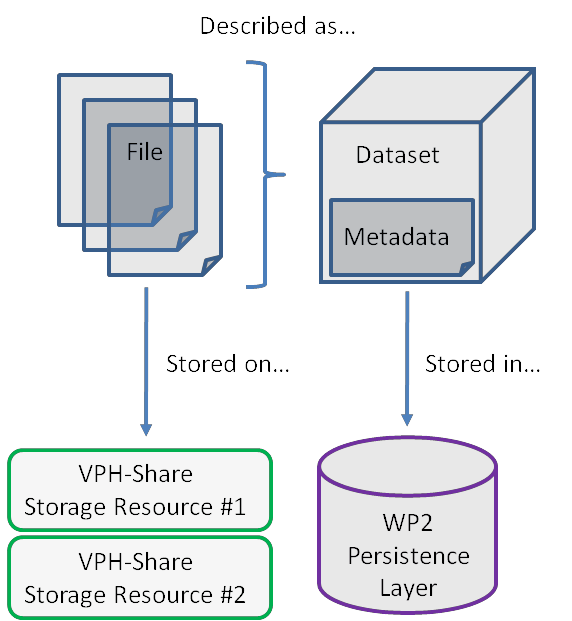
\includegraphics[scale=0.15]{img/managed-dataset.png}
			\hspace{1cm}
			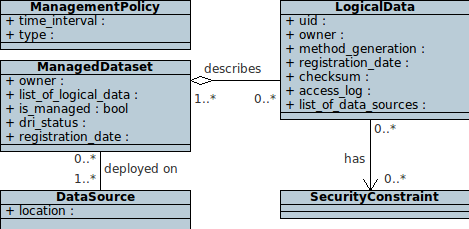
\includegraphics[scale=0.4]{img/data_model.png}
		\end{figure}
	\end{itemize}
	\item Data integrity requirements
	\begin{itemize}
		\item periodical and on-request monitoring of data availability and integrity
		\item network efficient validation algorithm
		\item data replication in federated cloud storage environment
	\end{itemize}
\end{itemize}
\end{block}
\end{frame}

%---------------------------------------------------------------------------

\begin{frame}
\frametitle{\hspace{5mm} \textbf{Objectives of this thesis}}
\begin{block}{}
\textbf{The main objective of this thesis is to create a~data reliability and integrity tool
(DRI) in form of a~web service that would monitor the availability and integrity of data stored
in federated cloud storage.}
\end{block}
\begin{block}{}
\textbf{Important aspects of this work} 
\begin{itemize}
	\item design and implementation of validation web service prototype
	\item integration of DRI service with the rest of VPH-Share project
	\item periodical and on-request validation
	\item literature research on efficient cloud storage validation algorithm
	\item propose network efficient validation algorithm of data in the cloud
\end{itemize}
\end{block}
\end{frame}

%---------------------------------------------------------------------------

\begin{frame}
\frametitle{\hspace{5mm} \textbf{Standard methods for data integrity}}
\begin{block}{}
\textbf{Data integrity building blocks:}
\begin{itemize}
	\item hash functions (MD5, SHA-1, SHA-256),
	\item Message Authentication Code(MAC) -- integrity and authenticity assurance
	\item Error Correcting Code(ECC) -- corruption detection and correction
\end{itemize}

\textbf{Popular approaches:}
\begin{itemize}
	\item MD5/SHA-1 checksum for software packages
	\item integrity checksums for network messages
	\item ECCs in hardware solution
\end{itemize}
\end{block}

\begin{block}{}
\textbf{Cloud storage data integrity challenges:}
\begin{itemize}
	\item huge amounts of data -- inefficient remote validation
	\item externallly stored over broadband network -- network limitations
\end{itemize}
\textbf{If whole-file content validation is infeasible, then maybe we should try probabilistic validation}
\end{block}
\end{frame}

%---------------------------------------------------------------------------

\begin{frame}
\frametitle{\hspace{5mm} \textbf{Approaches to data integrity in the cloud}}
\begin{block}{}
\begin{tabular}{l l}
	\begin{minipage}{0.4\textwidth}
  	\textbf{Proof of Retrievability (POR) scheme:}
	\begin{itemize}
		\item divide a~file $F$ into $b$ blocks and apply ECCs
		\item encrypt the file with appended parity bits
		\item select $m$ blocks out of $M$, compute MACs and append them to file
	\end{itemize}
	\end{minipage}
	&
	\begin{minipage}{0.6\textwidth}
		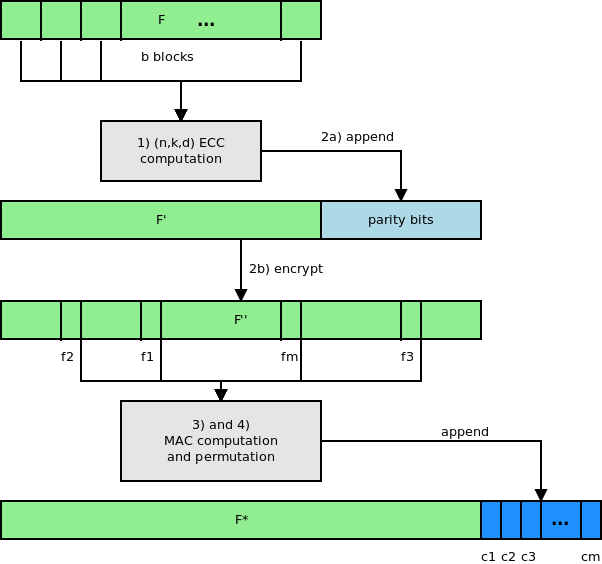
\includegraphics[width=0.5\paperwidth]{img/por-schematic.png}
	\end{minipage}
\end{tabular}
\end{block}
\end{frame}

%---------------------------------------------------------------------------

\begin{frame}
\frametitle{\hspace{5mm} \textbf{Approaches to data integrity in the cloud}}
\begin{block}{}
\begin{tabular}{l l}
	\begin{minipage}{0.4\textwidth}
	\textbf{Data integrity proofs (DIP) scheme:}
	\begin{itemize}
		\item divide a~file $F$ into $n$ blocks and select randomly $k$ bits from every block
		\item concatenate all selected bits and ecnrypt them
		\item append encrypted bits to the end of file
	\end{itemize}
	\end{minipage}
	&
	\begin{minipage}{0.6\textwidth}
		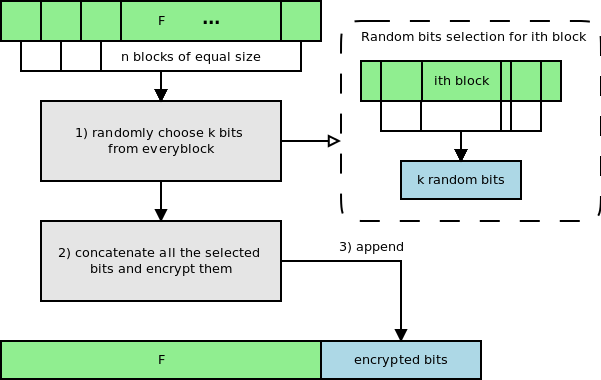
\includegraphics[width=0.5\paperwidth]{img/dip-schematic.png}
	\end{minipage}
\end{tabular}
\end{block}
\end{frame}

%---------------------------------------------------------------------------

\begin{frame}
\frametitle{\hspace{5mm} \textbf{Drawbacks of the outlined approaches}}
\begin{block}{}
	\begin{itemize}
		\item modifications applied to the original file (appending metadata, content encryption)
		\item assume computing capabilities on the prover side
		\item do not take into account cloud REST API limitations (no support for multiple HTTP Range requests)
	\end{itemize}
\end{block}
\end{frame}

%---------------------------------------------------------------------------

\begin{frame}
\frametitle{\hspace{5mm} \textbf{DRI service design}}
\begin{tabular}{l l}
	\begin{minipage}{0.35\textwidth}
	\begin{itemize}
		\item stateless REST web service in VPH-Share cloud environment
		\item periodical and on-request probabilistic validation of data in federated cloud storage
		\item data replication over cloud providers
	\end{itemize}
	\end{minipage}
	&
	\begin{minipage}{0.6\textwidth}
		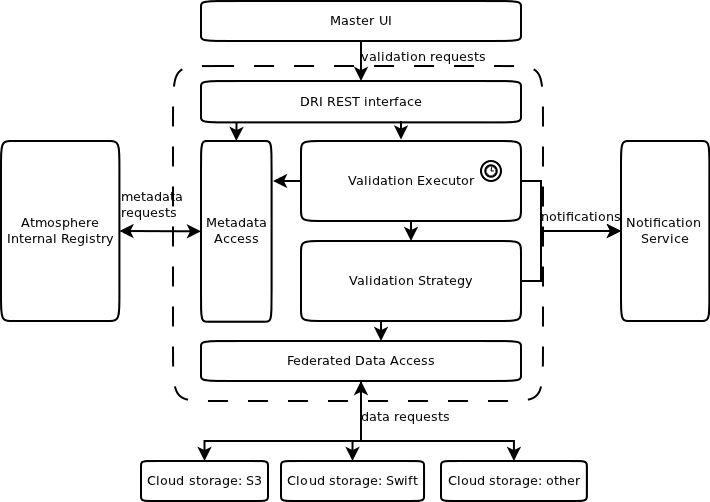
\includegraphics[width=0.6\paperwidth]{img/dri-architecture.png}
	\end{minipage}
\end{tabular}
\begin{tabular}{l l}
	\begin{minipage}{0.4\textwidth}
	\textbf{Implementation technologies}
	\begin{itemize}
		\item JClouds library -- cloud storage abstraction
		\item Quartz -- task scheduling
		\item JAX-RS -- REST web service
		\item Java, Guice, Guava, Tomcat
	\end{itemize}
	\end{minipage}
	&
	\begin{minipage}{0.6\textwidth}
		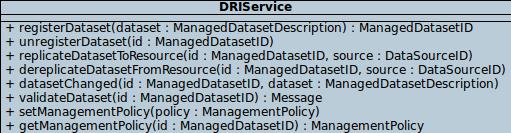
\includegraphics[width=0.6\paperwidth]{img/dri_interface.png}
	\end{minipage}
\end{tabular}
\end{frame}

%---------------------------------------------------------------------------

\begin{frame}
\frametitle{\hspace{5mm} \textbf{DRI validation algorithm}}
\begin{tabular}{l l}
	\begin{minipage}{0.4\textwidth}
	\textbf{Setup phase}
	\begin{itemize}
		\item divide file $F$ into $n$ equal chunks
		\item compute MAC checksum for every chunk and store
	\end{itemize}
	\textbf{Validation phase:}
	\begin{itemize}
		\item randomly select $k$ chunks
		\item compute MAC checksum of selected chunks and compare
	\end{itemize}
	\begin{table}[h!]
	\centering
	{\footnotesize
	\begin{tabular}{|l||c|c|}
		\hline
		Metric     & our approach                                           & whole-file approach \\ \hline \hline
		$E_{det}$  & ${k \over n}$                                          & 1 \\ \hline
		$N_{over}$ & $\sim F \times {k \over n}$                            & $\sim F$ \\ \hline
		$T_{exec}$ & $\sim k \times ({F \over {n \times speed}} + latency)$ & $\sim {F \over speed} + latency$ \\ \hline
	\end{tabular}
	}
	\end{table}
	\end{minipage}
	&
	\begin{minipage}{0.6\textwidth}
	\begin{figure}
		\centering
		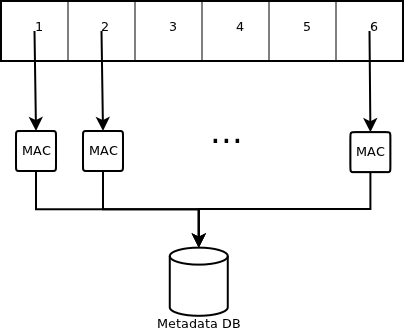
\includegraphics[width=0.5\textwidth]{img/algorithm-setup.png}
		\caption{Setup phase}
	\end{figure}
	\begin{figure}
		\centering
		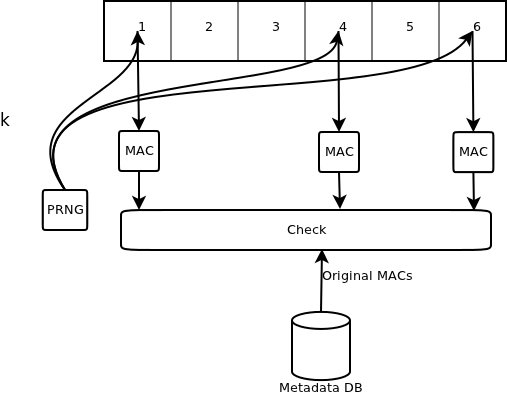
\includegraphics[width=0.5\textwidth]{img/algorithm-validation.png}
		\caption{Validation phase}
	\end{figure}
	\end{minipage}
\end{tabular}
\end{frame}

%---------------------------------------------------------------------------

\begin{frame}
\frametitle{\hspace{5mm} \textbf{DRI service verification}}
	\begin{figure}
		\centering
		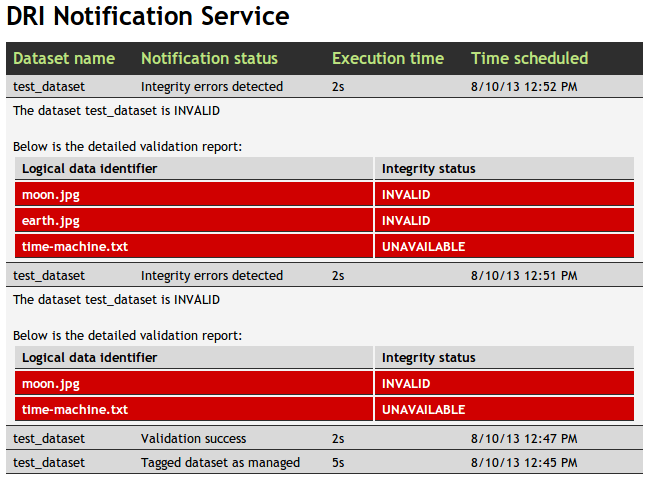
\includegraphics[width=0.75\textwidth]{img/test-scenario-results.png}
	\end{figure}
\end{frame}

%---------------------------------------------------------------------------

\begin{frame}
\frametitle{\hspace{5mm} \textbf{Results and future work}}
\begin{block}{}
\textbf{Results:}
\begin{itemize}
	\item proposed an efficient algorithm for data validation in the cloud
	\item proposed methodology to monitor data reliability and integrity in the cloud
	\item enabled VPH-Share project users to monitor data integrity and notify in case of failures
\end{itemize}
\end{block}
\begin{block}{}
\textbf{Future work:}
\begin{itemize}
	\item Design how to combine DRI monitoring service with federated cloud storage data access layer
	\item Extract DRI component from VPH-Share context and share as open source
	\item Design better data validation algorithm in the cloud
\end{itemize}
\end{block}
\end{frame}

\begin{frame}
\frametitle{\hspace{5mm} \textbf{Acknowledgement}}
More at \url{http://dice.cyfronet.pl/VPH-Share}\\

\begin{block}{}
\textbf{This thesis was realized partially in the framework of the following projects:}
\begin{itemize}
	\item Virtual Physiological Human: Sharing for Healthcare (VPH-Share) – partially funded by the European Commission under the Information Communication Technologies Programme (contract number 269978).
	\item Project UDA-POKL.04.01-01-00-367/08-00 "Improvement of didactic potential of computer science specialization at AGH", at the Department of Computer Science, AGH University of Science and Technology, Al. A. Mickiewicza 30, 30-059 Kraków
\end{itemize}
\end{block}
\begin{figure}[h!]
	\centering
	\begin{subfigure}[b]{0.3\textwidth}
		
\includegraphics[width=\textwidth, keepaspectratio=true]{img/kapital.png}
	\end{subfigure}
	\qquad
	\begin{subfigure}[b]{0.06\textwidth}
		
\includegraphics[width=\textwidth, keepaspectratio=true]{img/agh.png}
	\end{subfigure}
	\qquad
	\begin{subfigure}[b]{0.3\textwidth}
		
\includegraphics[width=\textwidth, keepaspectratio=true]{img/ue.png}
	\end{subfigure}
\end{figure}
\end{frame}



\end{document}

